\documentclass{beamer}
\usepackage{hyperref}
\usepackage{subfig}  %% Para incluir subgraficos
\usepackage{media9} % 
\usepackage{url}

\hypersetup{pdfstartview={Fit}, bookmarks=True, pdftitle={Wave Propagation Lectures},
            pdfauthor={Nicolas Guarin-Zapata}, pdfsubject={Lectures},
            pdfkeywords={Waves, Elasticity, Numerical Methods}}  % Configure hyperref

%--- New commands ----%
\newcommand{\footref}[1]{\textsuperscript{\ref{#1}}}
\newcommand{\pardiff}[2]{\frac{\partial #1}{\partial #2}}
\newcommand{\pardiffd}[2]{\frac{\partial^2 #1}{\partial #2^2}}
%---------------------%

%\usefonttheme[onlymath]{serif}  % Make equations to be in serif fonts
\usefonttheme{serif}  % Make equations to be in serif fonts

\begin{document}


%title
\title[Wave propagation in solids] % (optional, only for long titles)
{Wave propagation:}
\subtitle{Solid Mechanics}
\author[Guarin-Zapata, Nicolas] % (optional, for multiple authors)
{Nicol\'as Guar\'in Zapata\\ \texttt{\small nguarin@purdue.edu}\\
{\tiny Slides available at: \url{https://github.com/nicoguaro/CE597-slides}}}
\institute{Civil Engineering Department\\
  Purdue University}
\date{\today}
\subject{Wave propagation}

% Title page
\frame{\titlepage}

% Outline
\begin{frame}
	\frametitle{Outline}
	\tableofcontents
\end{frame}
%


% Introduction about waves in general
\section{Introduction}
\begin{frame}
\frametitle{Introduction}
A wave is the propagation of certain medium property perturbation, e.g., density, pressure, electric field or magnetic field, that travel through the space transporting energy. The perturbed medium could be of diverse nature like air, water, a piece of metal or vacuum.

The property that presents the phenomena is expressed as function of position and time $\psi(\vec{r},t)$. Mathematically  it is said that $\psi$ is a wave if it verifies the wave equation:
\[\nabla^2 \psi(\vec{r},t)= \frac{1}{v^2} \frac{\partial^2 }{\partial t^2}\psi(\vec{r},t) \enspace ,\]
where $v$ is the wave propagation speed. For instance, some perturbations of the pressure, called sound, verify the above equation.
\end{frame}

% Examples
\subsection{Examples}
\begin{frame}\frametitle{Global Seismic Wave Propagation Simulation}
\begin{figure}[H]
\centering
\includemedia[
  width=0.5\textwidth,
  height=0.5\linewidth,
  activate=pageopen,
  addresource=vids/global.flv,
  flashvars={source=vids/global.flv}
]{}{VPlayer.swf}
\caption{Global Seismic Wave Propagation Simulation.\footnote{Contributors from ICES, The University of Texas at Austin: Carsten Burstedde, Omar Ghattas, James R. Martin, Georg Stadler, Lucas C. Wilcox Visualization at the Texas Advanced Computing Center, the University of Texas at Austin by Greg Abram: \url{http://vimeo.com/30813579}}}
\label{vid:global}
\end{figure}
\end{frame}

\begin{frame}\frametitle{Global Seismic Wave Propagation Simulation}
\begin{figure}[H]
\centering
\includemedia[
  width=0.8\textwidth,
  height=0.45\linewidth,
  activate=pageopen,
  addresource=vids/asymmetric_cannon.flv,
  flashvars={source=vids/asymmetric_cannon.flv}
]{}{VPlayer.swf}
\caption{Vertical Plane SH wave in an asymmetric canyon.\footnote{Juan Diego Jaramillo et al. 2012}}
\label{vid:canyon}
\end{figure}
\end{frame}

\begin{frame}\frametitle{Scattering of a pressure wave around a long cylinder}
\begin{figure}[H]
\centering
\includemedia[
  width=0.8\textwidth,
  height=0.6\linewidth,
  activate=pageopen,
  addresource=vids/scat-cylinder.flv,
  flashvars={source=vids/scat-cylinder.flv}
]{}{VPlayer.swf}
\caption{Scattering of a pressure wave around a long cylinder }
\label{vid:cylinder}
\end{figure}
\end{frame}

% Wave characteristics
\section{Wave characteristics}
\begin{frame}
	\frametitle{Wave characteristics}
There are great variety of waves but all of them could experiment
\begin{itemize}
\item \textbf{Reflection}:Occurs when a wave find a new medium, that can not cross, change its direction.

\item \textbf{Refraction}: Occurs when a wave change its direction when enter in a new medium with different propagation speed.

\item \textbf{Doppler Effect}: Effect caused by the relative motion between the source and the receptor.

\item \textbf{Interference}: Occurs when two or more waves coexist in the same place and are superimposed.

\item \textbf{Diffraction}: Occurs when a wave find the border of an obstacle and change its \emph{form} to round it.
\end{itemize}

\end{frame}

% Waves in a string
\section{Waves in a string}
\subsection{Formulation}
\begin{frame}\frametitle{Waves in a string}
	
\transwipe
	
\begin{figure}[h]
	\centering
	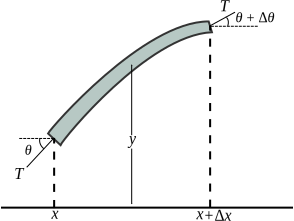
\includegraphics[height=4cm]{img/string.pdf}
	\caption{Forces diagram over an element of the string with length $\Delta x$. }
\end{figure}

\only<1> {For a string with length $L$, linear mass density $\mu$ and a tension $T$, let's take a small segment with small displacements in $y$. The force balance over the element showed in the Figure is:
\begin{align*}
F_y &= T \sin(\theta + \Delta \theta) - T \sin(\theta)\\
F_x &= T \cos(\theta + \Delta \theta) - T \cos(\theta) \enspace ,
\end{align*}}

\only<2>{Taking small displacements in the string, the angles are also small and then
\begin{align*}
F_y &\approx T (\theta + \Delta \theta) - T (\theta) = T \Delta \theta\\
F_x &\approx 0 \enspace .
\end{align*}}
\end{frame}

\begin{frame}[allowframebreaks]\frametitle{Waves in a string}		
From the second Newton's law we get
\[T\ \Delta \theta = \underbrace{(\mu\ \Delta x)}_\text{mass} a_y \enspace ,\]
if we take the limit $\Delta x \rightarrow dx$
\begin{equation}
T\ d\theta = (\mu\ dx) a_y \enspace .
\label{eq:stringForce}
\end{equation}
And we know that $\tan \theta = \frac{\partial y}{\partial x}$, taking derivative respect $x$
\[\sec^2 \theta \frac{d\theta}{dx} = \frac{\partial^2 y}{\partial x^2} \enspace .\]
Due to small displacements $\sec^2 \theta \approx 1$, hence
\begin{equation}
d\theta \approx \frac{\partial^2 y}{\partial x^2} dx
\label{eq:stringDtheta}
\end{equation}
and replacing (\ref{eq:stringDtheta}) in  (\ref{eq:stringForce})
\[T \frac{\partial^2 y}{\partial x^2} dx = (\mu\ dx) \frac{\partial^2 y}{\partial t^2} \enspace ,\]
we finally get the 1D Wave Equation
\[\frac{\partial^2 y}{\partial x^2} = \frac{\mu}{T} \frac{\partial^2 y}{\partial t^2} \enspace .\]

$T/\mu$ have square speed units, and is the square propagation speed
\[v = \sqrt{\frac{T}{\mu}} \enspace ,\]
so
\begin{equation}
\frac{\partial^2 y}{\partial x^2} = \frac{1}{v^2} \frac{\partial^2 y}{\partial t^2} \enspace .
\label{eq:wave_eq}
\end{equation}

\end{frame}


% Solution for the 1D Case
\subsection{Solution}
\begin{frame}[allowframebreaks]\frametitle{Solution for the 1D case}
	
The wave equation could be solved by separation of variables, i.e., let's suppose it has a solution of the form $y=y(x,t)=X(x)T(t)=X\ T$
\[\frac{1}{X} \frac{d^2 X}{dx^2} - \frac{1}{v^2 T} \frac{d^2 T}{dt^2} = 0 \enspace ;\]
we can see that the temporal and the spatial terms are isolated, so they should be equal to a constant. For simplicity let's take $-\alpha^2$, with $\alpha\in \mathbb{R}$
\[\frac{d^2 X}{dx^2}=-\alpha^2 X, \qquad \frac{d^2 T}{dt^2}=-\alpha^2 v^2 T \enspace ,\]
so the solution is
\[y = \left[C_1 \sin(\alpha x)+ C_2\cos(\alpha x) \right] \left[C_3\sin(\alpha v t) +C_4 \cos(\alpha v t)\right] \enspace .\]
If we take fixed extremes and assume that the string starts with a deformed shape $f(x)$, i.e., $y(0,t)=y(L,t)$, $y(x,0)=f(x)$ and $y'(x,0)=0$ can be shown that the complete solution is
\[y(x,t) = \frac{2}{L}\sum\limits_{n=1}^{\infty}\left[\int\limits_{0}^{L}f(\xi)\sin\left(\frac{n\pi\xi}{L}\right)d\xi\right] \sin\left(\frac{n\pi x}{L}\right)\cos\left(\frac{n\pi v t}{L}\right) \enspace .\] 
\end{frame}

\subsection{An example}
\begin{frame}\frametitle{Example in 1D}
% Encoding for media9: ffmpeg -i movie.avi -sameq movie.flv  or
%                      ffmpeg -i movie.avi -sameq -vcodec libx264 -x264opts keyint=25 movie.mp4
\begin{figure}[H]
\centering
\includemedia[
  width=0.8\textwidth,
  height=0.6\linewidth,
  activate=pageopen,
  addresource=vids/ex1D.flv,
  flashvars={source=vids/ex1D.flv}
]{}{VPlayer.swf}
\caption{Wave traveling in a string.}
\label{vid:string}
\end{figure}
\end{frame}


% Speed Wavelength and Frequency
\begin{frame}\frametitle{Wavelength}
Once the speed of propagation is known, the frequency of the sound produced by the string can be calculated. The speed of propagation of a wave is equal to the wavelength $\lambda$ divided by the period $\tau$, or multiplied by the frequency $f$:
\[v \equiv \sqrt{\frac{T}{\mu}} =\frac{\lambda}{\tau} = \lambda f \enspace .  \]	
\begin{figure}[h]
	\centering
	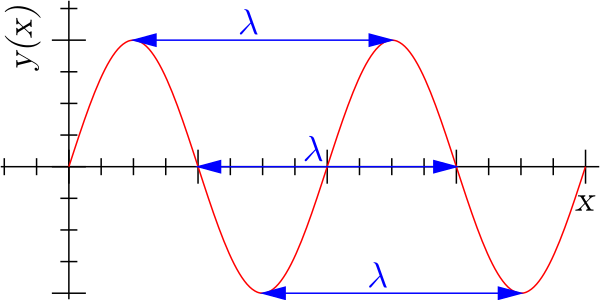
\includegraphics[height=3cm]{img/Sine_wavelength.pdf}
	\caption{Wavelength of a sine wave, $\lambda$, can be measured between any two points with the same phase, such as between crests, or troughs, or corresponding zero crossings as shown.}
\end{figure}
\end{frame}

%% Elastic waves
\section{Elastic waves}
\subsection{Starting point}
\begin{frame}\frametitle{Navier-Cauchy Equations: Starting Point}
In a three dimensional solid we can describe waves starting from the continuity equation, motion equations and constitutive relationships.
\begin{itemize}
\item Continuity:
\[\frac{\partial}{\partial t}\rho = - \frac{\partial}{\partial x_i}\left( \rho \frac{\partial}{\partial t} u_i\right)\]

\item Equations of Motion:
\[ \frac{\partial^2}{\partial t^2}(\rho u_i) = \frac{\partial}{\partial x_j} \sigma_{ij} + f_i \]

\item Constitutive relationships:
\[\sigma_{ij} = C_{ijkl} \epsilon_{kl}  \enspace ,\]

\end{itemize}
where $u_i$ is the displacement of a material point in $i$ direction, $\rho$ is the mass density, $\sigma_{ij}$ the stress tensor, $\epsilon_{kl}$ is the strain tensor, $f_i$ are \emph{body forces} and $C_{ijkl}$ depends on the material of the medium.
\end{frame}

% continuity equation
\subsubsection{Continuity equation}
\begin{frame}[allowframebreaks]\frametitle{Continuity equation}
\begin{figure}[h]
	\centering
	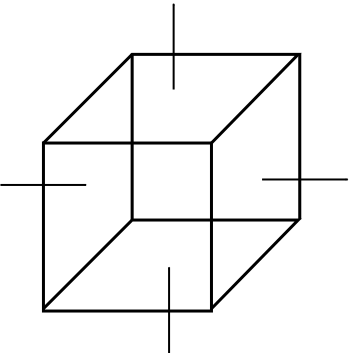
\includegraphics[height=6cm]{img/continuity.pdf}
	\caption{Fluxes on a parallelepiped element.}
\end{figure}
The total mass of the element is $M_T = \rho dx\, dy\, dz$, and its rate is
\[\pardiff{M_T}{t} = \pardiff{\rho}{t} dx\, dy\, dz \enspace .\]
We can compute the total flow through the $x$ direction:
\[\left[ \rho \pardiff{u_1}{t} + \pardiff{}{x}\left(\rho \pardiff{u_1}{t}\right) dx\right] dy\, dz - \rho \pardiff{u_1}{t} dy\, dz = \pardiff{}{x}\left(\rho \pardiff{u_1}{t}\right)dx\, dy\, dz \enspace .\]
Similarly, for the other directions
\[\pardiff{}{y}\left(\rho \pardiff{u_2}{t}\right)dx\, dy\, dz,\qquad \pardiff{}{z}\left(\rho \pardiff{u_3}{t}\right)dx\, dy\, dz \enspace ,\]
and equating to the first expression
\[\pardiff{\rho}{t} + \pardiff{}{x}\left(\rho \pardiff{u_1}{t}\right) + \pardiff{}{y}\left(\rho \pardiff{u_2}{t}\right) + \pardiff{}{z}\left(\rho \pardiff{u_3}{t}\right) = 0\enspace .\]
In index notation
\[\pardiff{\rho}{t} = - \pardiff{}{x_i}\left(\rho \pardiff{u_i}{t}\right) \quad \text{Summation over } i \enspace ,\]
and, in vector notation
\[\pardiff{\rho}{t} = - \nabla \cdot \left(\rho \pardiff{\vec{u}}{t}\right) \enspace.\]
\end{frame}

% Balance of momentum
\subsubsection{Balance of momentum}
\begin{frame}[allowframebreaks]\frametitle{Balance of momentum: ``Equations of Motion"}
\begin{figure}[h]
	\centering
	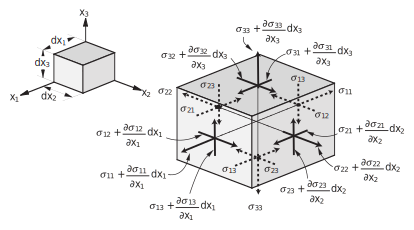
\includegraphics[height=6cm]{img/momentum.pdf}
	\caption{Stresses on a parallelepiped element.}
\end{figure}
We are going to do the balance of forces in the $x_1$ direction
\begin{align*}
\rho \pardiffd{u_1}{t} dx\, dy\, dz =& \left(\sigma_{11} + \pardiff{\sigma_{11}}{x_1}dx_1\right)dx_2\, dx_3 - \sigma_{11} dx_2\, dx_3\\
&+ \left(\sigma_{21} + \pardiff{\sigma_{21}}{x_2}dx_2\right)dx_1\, dx_3
 -\sigma_{21}dx_1\, dx_3\\
&+ \left(\sigma_{31} + \pardiff{\sigma_{31}}{x_3}dx_3\right)dx_1\, dx_2\\
&- \sigma_{31}dx_1\, dx_2 + f_1 dx_1\, dx_2\, dx_3 \\
=& \left(\pardiff{\sigma_{11}}{x_1} + \pardiff{\sigma_{21}}{x_2} + \pardiff{\sigma_{31}}{x_3}\right)dx_1\, dx_2\, dx_3
\end{align*}
upon dividing by $dx_1\, dx_2\, dx_3$ we obtain
\[\pardiff{\sigma_{11}}{x_1} + \pardiff{\sigma_{21}}{x_2} + \pardiff{\sigma_{31}}{x_3} + f_1= \rho \pardiffd{u_1}{t} \enspace ,\]
similarly in the other two directions
\begin{align*}
\pardiff{\sigma_{12}}{x_1} + \pardiff{\sigma_{22}}{x_2} + \pardiff{\sigma_{32}}{x_3} =& \rho \pardiffd{u_3}{t} \\
\pardiff{\sigma_{13}}{x_1} + \pardiff{\sigma_{23}}{x_2} + \pardiff{\sigma_{33}}{x_3} =& \rho \pardiffd{u_3}{t} \enspace .
\end{align*}
In index notation
\[\pardiff{\sigma_{ji}}{x_j} + f_i = \rho\pardiffd{u_i}{t}\qquad \text{Summation over } j \enspace ,\]
and in vector notation
\[\nabla\cdot \sigma + \vec{f} = \rho \pardiffd{\vec{u}}{t} \enspace .\]
\end{frame}

\begin{frame}[allowframebreaks]\frametitle{Navier-Cauchy Equations: Deduction}
For an isotropic medium the constitutive relation can be expressed as
\[\sigma_{ij} = \lambda \delta_{ij}\epsilon_{kk} + 2\mu \epsilon_{ij} \enspace ,\]
being $\lambda$ and $\mu$ the Lame parameters.

$\epsilon_{ij}$ is usually define as
\[\epsilon_{ij} = \frac{1}{2} \left( \pardiff{u_i}{x_j} + \pardiff{u_j}{x_i} \right) \enspace ,\]
so
\[\sigma_{ij} = \lambda \delta_{ij} \pardiff{u_k}{x_k} + \mu \left( \pardiff{u_i}{x_j} + \pardiff{u_j}{x_i} \right) \enspace .\]

If we take the constitutive equation and replace $\sigma_{ij}$ in the motion equation (assuming that $\pardiff{\rho}{t}=0$).
\[\rho \pardiff{u_i}{t} = \delta_{ij} \lambda \pardiff{\epsilon_{kk}}{x_j} + 2\mu \pardiff{\epsilon_{ij}}{x_j} +f_i \enspace ,\]
and rewriting the right hand side in terms of the displacements we have
\[\rho \pardiff{^2 u_i}{t^2} = \delta_{ij} \lambda \pardiff{}{x_j}\left( \pardiff{u_k}{x_k}\right) + \mu \pardiff{ }{x_j}\left( \pardiff{u_i}{x_j} + \pardiff{u_j}{x_i}\right) + f_i \enspace ,\]
operating the Kronecker's delta
\[\rho \pardiff{^2 u_i}{t^2} = \lambda \pardiff{}{x_i}\left( \pardiff{u_k}{x_k}\right) + \mu \pardiff{}{x_j}\left( \pardiff{u_i}{x_j} + \pardiff{u_j}{x_i} \right) + f_i \enspace ,\]
and this can be rewritten like
\[\rho \pardiff{^2 u_i}{t^2} = \lambda  \pardiff{^2 u_j}{x_i x_j} + \mu \pardiff{^2 u_i}{x_j^2} + \mu \pardiff{^2 u_j}{x_j x_i} + f_i \enspace ,\]
grouping terms
\begin{equation}
\rho \pardiff{^2 u_i}{t^2} = (\lambda + \mu)  \pardiff{}{x_i}\left( \pardiff{u_j}{x_j} \right) + \mu \pardiff{^2 u_i}{x_j^2}  + f_i \enspace .
\label{eq:navierInd}
\end{equation}
This is the Navier Equation that can be expressed also in vector form
\[\rho \pardiff{^2 u_i}{t^2} = (\lambda + \mu)  \underbrace{\pardiff{}{x_i}}_{\mbox{grad}}\nabla \cdot \vec{u} + \mu \nabla^2 u_i + f_i \enspace ,\]
or
\begin{equation}
\rho \pardiff{^2 \vec{u}}{t^2} = (\lambda + \mu)  \nabla (\nabla\cdot \vec{u})+ \mu \nabla^2 \vec{u} + \vec{f} \enspace .
\label{eq:navierVec}
\end{equation}
The body forces will be neglected hereinafter for simplicity. The vector 
\[\nabla^2 \vec{a} = \nabla (\nabla \cdot \vec{a}) - \nabla \times (\nabla \times \vec{a}) \enspace ,\]
identity is used, and we get
\[\rho \pardiff{^2 \vec{u}}{t^2} = (\lambda + 2\mu) \nabla(\nabla \cdot \vec{u}) - \mu (\nabla \times (\nabla \times \vec{u})) \enspace .\]
If we take $\varphi = \nabla \cdot \vec{u} $ and $\vec{\psi} = \nabla \times \vec{u}$ and replace it in the Navier equation we obtain:
\begin{equation}
\rho \pardiff{^2 \vec{u}}{t^2} = (\lambda + 2\mu) \nabla \varphi - \mu \nabla \times \vec{\psi} \enspace .
\label{eq:waveHelm}
\end{equation}
\end{frame} 

% P-waves
\subsection{P-waves equation}
\begin{frame}\frametitle{P-waves equation}
Taking divergence to (\ref{eq:waveHelm})
\[\nabla\cdot \left( \pardiff{^2 \vec{u}}{t^2} \right)= (\lambda +2\mu) \nabla\cdot \nabla \varphi - \mu\nabla\cdot\nabla\times \vec{\psi} \enspace , \]
we finally get
\begin{equation}
\nabla^2 \varphi = \frac{1}{\frac{\lambda + 2\mu}{\rho}} \pardiff{^2 \varphi}{t^2} \enspace ,
\label{eq:pWave}
\end{equation}
with speed of propagation
\[v_P := \sqrt{\frac{\lambda + 2\mu}{\rho}}\]
\end{frame}

\begin{frame}\frametitle{P-wave polarization}
\begin{figure}[H]
\centering
\includemedia[
  width=0.8\textwidth,
  height=0.6\linewidth,
  activate=pageopen,
  addresource=vids/P-0.flv,
  flashvars={source=vids/P-0.flv}
]{}{VPlayer.swf}
\caption{Particle motion in a P wave.}
\label{vid:P0}
\end{figure}
\end{frame}

% S-waves
\subsection{S-waves equation}
\begin{frame}\frametitle{S-waves equation}
Taking rotational to (\ref{eq:waveHelm})
\[\nabla\times \left( \pardiff{^2 \vec{u}}{t^2} \right)= (\lambda +2\mu) \nabla\times \nabla \varphi - \mu\nabla\times\nabla\times \vec{\psi} \enspace , \]
we finally get
\begin{equation}
\nabla^2 \vec{\psi} = \frac{1}{\frac{\mu}{\rho}} \pardiff{^2 \vec{\psi}}{t^2} \enspace ,
\label{eq:SWave}
\end{equation}
with speed of propagation
\[v_S := \sqrt{\frac{\mu}{\rho}}\]
\end{frame}

\begin{frame}\frametitle{S-wave polarization}
\begin{figure}[H]
\centering
\includemedia[
  width=0.8\textwidth,
  height=0.6\linewidth,
  activate=pageopen,
  addresource=vids/SV-0.flv,
  flashvars={source=vids/SV-0.flv}
]{}{VPlayer.swf}
\caption{Particle motion in a SV wave.}
\label{vid:SV0}
\end{figure}
\end{frame}

%
\begin{frame}\frametitle{References}
\begin{itemize}
\item Michael A. Slawinski. Waves and rays in Elastic Continua. Second Edition, 2007.
 
\item Wikipedia community. Onda (f\'isica) [on line]. Wikipedia, La enciclopedia libre, 2010 ; 22 November 2010. 

\item George B. Arfken \& Hans. J. Weber. Mathematical Methods for Physicists. Elsevier Academic Press, 6th Edition, San Diego, 2005.
\end{itemize}
\end{frame}



\end{document}

